\documentclass[12pt,a4paper]{article}
\usepackage[utf8]{vietnam}
\usepackage{amsmath,amssymb}
\usepackage{geometry}
\geometry{top=1.5cm,bottom=1.2cm,left=1.4cm,right=1.4cm,headheight=28pt,headsep=12pt,footskip=18pt}
\usepackage{tikz}
\usepackage{xcolor}
\usepackage{enumerate}
\usepackage{graphicx}
\usepackage[version=4]{mhchem}
\usepackage{fancyhdr}
\usepackage{ex_test}

\renewcommand{\baselinestretch}{0.96}
\setlength{\parskip}{0pt}

\definecolor{hfRed}{RGB}{211,47,47}
\definecolor{hfGreen}{RGB}{139,195,144}

\providecommand{\False}{}

\pagestyle{fancy}
\fancyhf{}
\fancyhead[L]{\small\itshape\color{hfRed} Tài liệu lưu hành nội bộ}
\fancyhead[R]{\small\itshape\color{hfRed} Thầy \textbf{TRẦN VĂN THẠNH} - 0777.470.803}
\renewcommand{\headrulewidth}{0.8pt}
\renewcommand{\headrule}{\hbox to\headwidth{\color{hfGreen}\leaders\hrule height \headrulewidth\hfill}}

\fancyfoot[L]{\small\itshape\color{hfRed} CS1: 6/15 Nguyễn Hoàng, P. Kim Long, TP Huế \quad|\quad CS2: 24 Đặng Thái Thân, TP Huế}
\fancyfoot[R]{\small\bfseries\color{hfRed} Trang \thepage}
\renewcommand{\footrulewidth}{0.8pt}
\renewcommand{\footrule}{\hbox to\headwidth{\color{hfGreen}\leaders\hrule height \footrulewidth\hfill}}

\fancypagestyle{firstpage}{
  \fancyhf{}
  \renewcommand{\headrulewidth}{0pt}
  \fancyfoot[L]{\small\itshape\color{hfRed} CS1: 6/15 Nguyễn Hoàng, P. Kim Long, TP Huế \quad|\quad CS2: 24 Đặng Thái Thân, TP Huế}
  \fancyfoot[R]{\small\bfseries\color{hfRed} Trang \thepage}
  \renewcommand{\footrulewidth}{0.8pt}
  \renewcommand{\footrule}{\hbox to\headwidth{\color{hfGreen}\leaders\hrule height \footrulewidth\hfill}}
}

\begin{document}
\thispagestyle{firstpage}

\noindent
\begin{minipage}[t]{0.44\textwidth}
	\centering\fontsize{10pt}{12pt}\selectfont
	\textbf{SỞ GIÁO DỤC VÀ ĐÀO TẠO THỪA THIÊN HUẾ}\\
	\textbf{ĐỀ CHÍNH THỨC}\\
	\textit{(Đề thi có 04 trang)}
\end{minipage}\hfill
\begin{minipage}[t]{0.54\textwidth}
	\centering\small
	\textbf{ĐỀ KIỂM TRA ĐỊNH KỲ CHƯƠNG 1 (ESTER -- LIPID)}\\
	\textbf{MÔN: HOÁ HỌC -- LỚP 12}\\
	\textit{Thời gian làm bài: 50 phút (không kể thời gian phát đề)}\\
	\fbox{\textbf{MÃ ĐỀ: 103}}
\end{minipage}

\smallskip
\noindent\hrulefill
\smallskip

\noindent\textbf{Họ, tên thí sinh:} \dotfill\ \textbf{Lớp:} \dotfill\ \textbf{Số báo danh:} \dotfill

\smallskip
\noindent\textit{(Cho biết nguyên tử khối: H = 1; C = 12; N = 14; O = 16; Na = 23; K = 39; Br = 80; Cl = 35,5).}
\smallskip

\noindent
\textbf{PHẦN I (4,5 điểm -- 18 câu): Câu trắc nghiệm nhiều phương án lựa chọn.}\\
\textit{Thí sinh trả lời từ câu 1 đến câu 18. Mỗi câu hỏi thí sinh chỉ chọn một phương án.}

\Opensolutionfile{ans}[ans-de03hs]

\begin{ex}
(SBT - KNTT). Chất nào sau đây thuộc loại ester?
\choice
{$\ce{HCOOCH3}$}
{$\ce{CH3COOH}$}
{$\ce{HCOOH}$}
{$\ce{CH3COCH3}$}
\loigiai{}
\end{ex}

\begin{ex}
(SBT - KNTT, CTST). Số đồng phân cấu tạo của ester có công thức $\ce{C4H8O2}$ là
\choice
{2}
{3}
{4}
{5}
\loigiai{}
\end{ex}

\begin{ex}
(SBT - KNTT). Ethyl propanoate là ester tạo nên mùi thơm đặc trưng của quả dứa. Công thức của ethyl propanoate là
\choice
{$\ce{CH3COOC2H5}$}
{$\ce{C2H5COOCH2CH2CH3}$}
{$\ce{CH3COOCH2CH2CH3}$}
{$\ce{C2H5COOC2H5}$}
\loigiai{}
\end{ex}

\begin{ex}
Ester nào sau đây tác dụng với dung dịch $\ce{NaOH}$ thu được sodium formate?
\choice
{$\ce{C2H5COOC2H5}$}
{$\ce{CH3COOC2H5}$}
{$\ce{CH3COOCH3}$}
{$\ce{HCOOCH3}$}
\loigiai{}
\end{ex}

\begin{ex}
Khi đun nóng chất X có công thức phân tử $\ce{C3H6O2}$ với dung dịch $\ce{NaOH}$ thu được $\ce{CH3COONa}$. Công thức cấu tạo của X là
\choice
{$\ce{CH3COOC2H5}$}
{$\ce{HCOOC2H5}$}
{$\ce{CH3COOCH3}$}
{$\ce{C2H5COOH}$}
\loigiai{}
\end{ex}

\begin{ex}
Chất nào sau đây phản ứng với dung dịch $\ce{NaOH}$ tạo thành $\ce{HCOONa}$ và $\ce{C2H5OH}$?
\choice
{$\ce{HCOOC2H5}$}
{$\ce{CH3COOC2H5}$}
{$\ce{CH3COOCH3}$}
{$\ce{HCOOCH3}$}
\loigiai{}
\end{ex}

\begin{ex}
(SBT - CTST). Tính chất nào sau đây không phải là tính chất thích hợp giúp ethyl methanoate ($\ce{HCOOC2H5}$) được sử dụng trong sản xuất một số loại nước hoa?
\choice
{Khả năng dễ cháy}
{Có mùi thơm dễ chịu}
{Không độc hại}
{Nhiệt độ sôi thấp}
\loigiai{}
\end{ex}

\begin{ex}
Nguyên liệu nào sau đây là nguyên liệu vô cơ chủ yếu trong phản ứng xà phòng hoá?
\choice
{Calcium hydroxide $\ce{Ca(OH)2}$}
{Sodium hydroxide $\ce{NaOH}$}
{Barium hydroxide $\ce{Ba(OH)2}$}
{Iron(III) hydroxide $\ce{Fe(OH)3}$}
\loigiai{}
\end{ex}

\begin{ex}
Xà phòng được tổng hợp theo phản ứng:
\begin{center}
	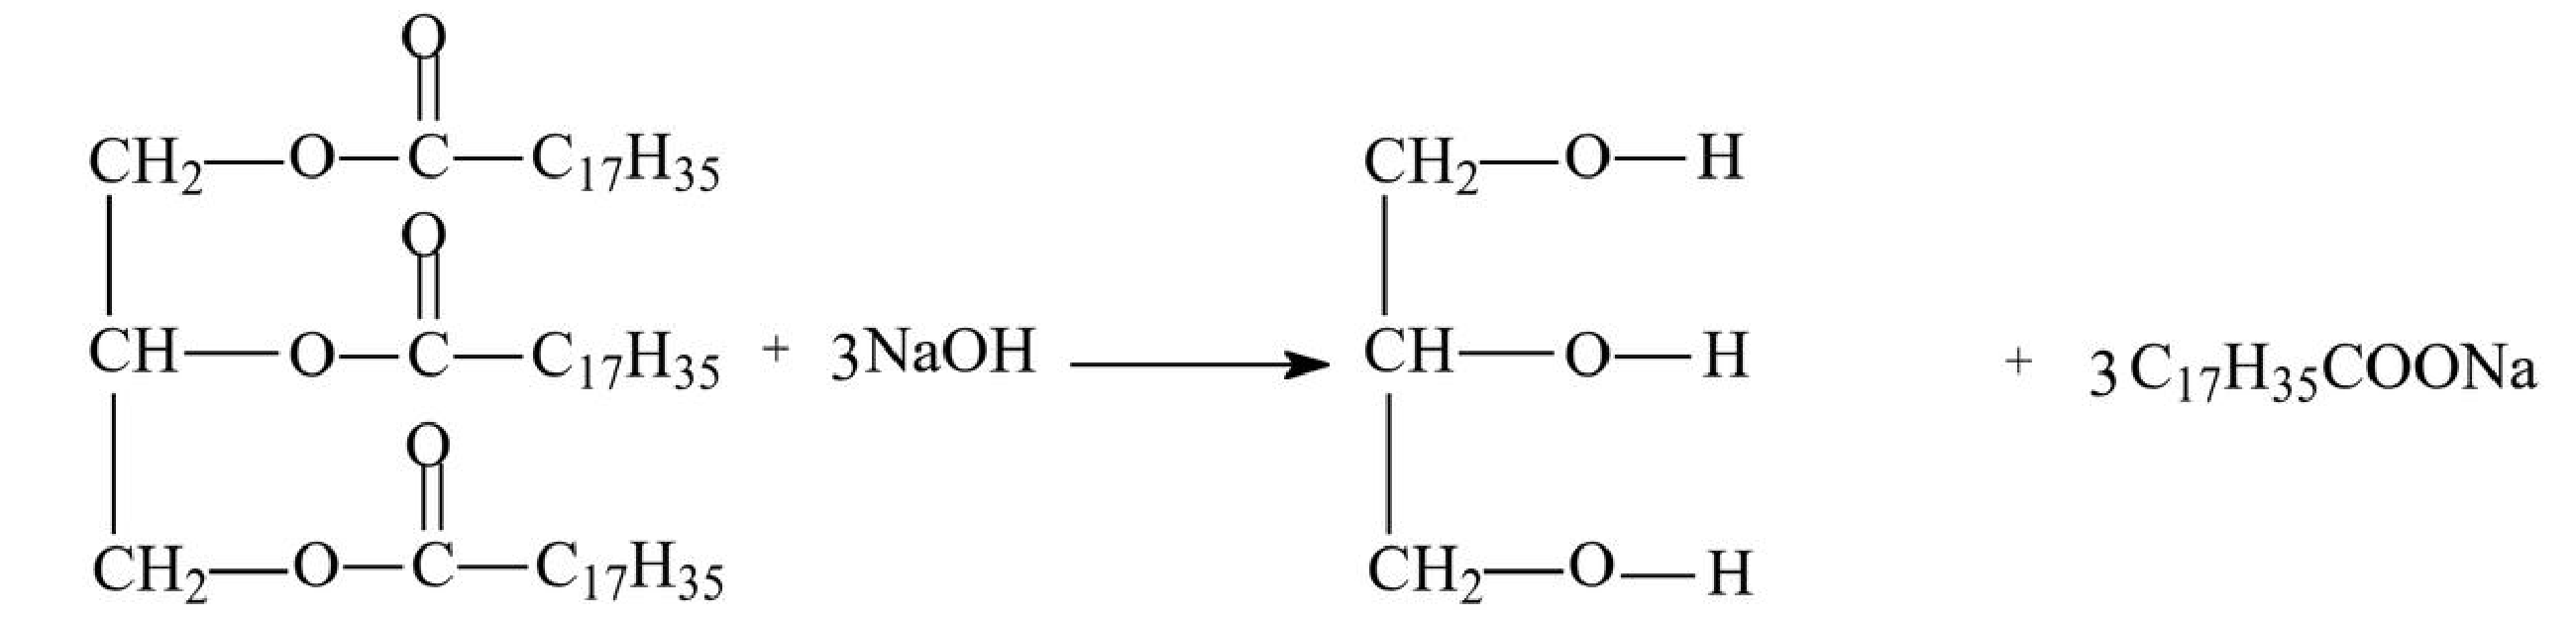
\includegraphics[width=12cm]{images_crop_de03/cau9_phan_ung_xa_phong_hoa.png}
\end{center}
Phản ứng trên là ví dụ của
\choice
{phản ứng ngưng tụ}
{phản ứng ester hóa}
{phản ứng oxi hóa}
{phản ứng thủy phân}
\loigiai{}
\end{ex}

\begin{ex}
Phát biểu nào sau đây không đúng?
\choice
{Chất béo không tan trong nước, nhẹ hơn nước nhưng tan nhiều trong dung môi hữu cơ}
{Dầu ăn và mỡ bôi trơn có cùng thành phần nguyên tố}
{Chất béo là triester của glycerol với các monocarboxylic acid có số chẵn nguyên tử carbon (12 - 24), mạch carbon dài, không phân nhánh}
{Phản ứng thủy phân chất béo trong môi trường base là phản ứng một chiều}
\loigiai{}
\end{ex}

\begin{ex}
Nguyên nhân nào làm cho bồ kết có khả năng giặt rửa:
\choice
{Vì bồ kết có những chất có cấu tạo kiểu đầu phân cực gắn với đuôi không phân cực}
{Vì bồ kết có thành phần là este của glycerine}
{Vì trong bồ kết có những chất oxi hóa mạnh}
{Vì trong bồ kết có chất khử mạnh}
\loigiai{}
\end{ex}

\begin{ex}
Cho phản ứng ester hóa: $\ce{RCOOH + R^{\prime}OH <=>[\ce{H2SO4},\, t^\circ] RCOOR^{\prime} + H2O}$. Để phản ứng chuyển dịch ưu tiên theo chiều thuận người ta thường:
\choice
{Dùng $\ce{H2SO4}$ đặc để hút nước và làm xúc tác}
{Chưng cất để tách ester ra khỏi hỗn hợp phản ứng}
{Tăng nồng độ của acid hoặc alcohol}
{Tất cả đều đúng}
\loigiai{}
\end{ex}

\begin{ex}
(SBT-CD). Phát biểu nào sau đây là không đúng?
\choice
{So với các đồng phân là carboxylic acid, ester luôn có nhiệt độ sôi thấp hơn}
{Phản ứng ester hoá là phản ứng thuận nghịch}
{Phản ứng xà phòng hoá là phản ứng thuận nghịch}
{Ester là những chất lỏng hoặc chất rắn ở nhiệt độ thường}
\loigiai{}
\end{ex}

\begin{ex}
Thủy phân ester có công thức $\ce{C4H8O2}$ (với xúc tác acid), thu được hai sản phẩm hữu cơ X và Y. Từ X có thể điều chế trực tiếp ra Y. Vậy chất X là:
\choice
{Methyl alcohol}
{Ethyl acetate}
{Formic acid}
{Ethyl alcohol}
\loigiai{}
\end{ex}

\begin{ex}
(SBT-CD). Thuỷ phân ester E có công thức phân tử $\ce{C4H8O2}$ với xúc tác acid vô cơ loãng, thu được hai sản phẩm hữu cơ X, Y (chỉ chứa các nguyên tử C, H, O). Từ X có thể điều chế trực tiếp ra Y bằng một phản ứng duy nhất. Chất X là chất nào sau đây?
\choice
{Acetic acid}
{Ethyl alcohol}
{Ethyl acetate}
{Formic acid}
\loigiai{}
\end{ex}

\begin{ex}
(SGK - KNTT). Cho các phát biểu sau:\\
(1) Một số ester có mùi thơm nên được dùng làm chất tạo hương trong công nghiệp thực phẩm và mĩ phẩm.\\
(2) Chất béo là triester của glycerol với acid béo.\\
(3) Chất béo tan tốt trong nước.\\
(4) Mỡ động vật, dầu thực vật có thể được dùng làm nguyên liệu để sản xuất xà phòng.\\
(5) Phản ứng thuỷ phân ester trong môi trường acid luôn là phản ứng một chiều.\\
Số phát biểu đúng là
\choice
{2}
{3}
{4}
{5}
\loigiai{}
\end{ex}

\begin{ex}
(SBT-CD). Tiến hành thí nghiệm điều chế isoamyl acetate (chất có mùi chuối chín) theo thứ tự các bước sau đây:\\
Bước 1: Cho khoảng $3\text{ mL}$ $\ce{CH3CH(CH3)CH2CH2OH}$, $3\text{ mL}$ $\ce{CH3COOH}$ và vài giọt $\ce{H2SO4}$ đặc vào ống nghiệm.\\
Bước 2: Lắc đều ống nghiệm rồi đun cách thuỷ (trong nồi nước nóng) khoảng 5--7 phút ở $65-70^\circ\text{C}$.\\
Bước 3: Làm lạnh, sau đó thêm khoảng $5\text{ mL}$ dung dịch $\ce{NaCl}$ bão hoà vào ống nghiệm.\\
Cho các phát biểu sau:\\
(a) $\ce{H2SO4}$ đặc có vai trò xúc tác cho phản ứng tạo isoamyl acetate.\\
(b) Thêm dung dịch $\ce{NaCl}$ bão hoà vào để tránh phân huỷ sản phẩm.\\
(c) Sau bước 2, trong ống nghiệm vẫn còn $\ce{CH3CH(CH3)CH2CH2OH}$ và $\ce{CH3COOH}$.\\
(d) Sau bước 3, trong ống nghiệm thu được hỗn hợp chất lỏng đồng nhất.\\
Số phát biểu đúng là
\choice
{4}
{5}
{3}
{2}
\loigiai{}
\end{ex}

\begin{ex}
Một loại chất béo có chứa 65\% tripalmitin về khối lượng. Để sản xuất 3 triệu hộp kem dưỡng da (có chứa chất dưỡng ẩm glycerol) cần dùng tối thiểu $x\text{ tấn}$ loại chất béo trên cho phản ứng với dung dịch $\ce{NaOH}$, đun nóng. Biết hiệu suất phản ứng đạt 80\%. Biết rằng trong mỗi hộp kem dưỡng da có chứa $5\text{ gam}$ glycerol. Giá trị của $x$ là
\choice
{152{,}7}
{525{,}4}
{252{,}7}
{175{,}7}
\loigiai{}
\end{ex}

\Closesolutionfile{ans}

\vspace{0.3cm}
\noindent
\textbf{PHẦN II (4,0 điểm -- 4 câu): Câu trắc nghiệm đúng sai.}\\
\textit{Thí sinh trả lời từ câu 1 đến câu 4. Trong mỗi ý a), b), c), d) ở mỗi câu, thí sinh chọn đúng hoặc sai.}

\setcounter{ex}{0}

\begin{ex}
Nhiều loại bơ thực vật (chất béo no ở dạng rắn) được tạo ra bởi quá trình hydrogen hóa một phần dầu thực vật (chất béo không no ở dạng lỏng).
\begin{center}
	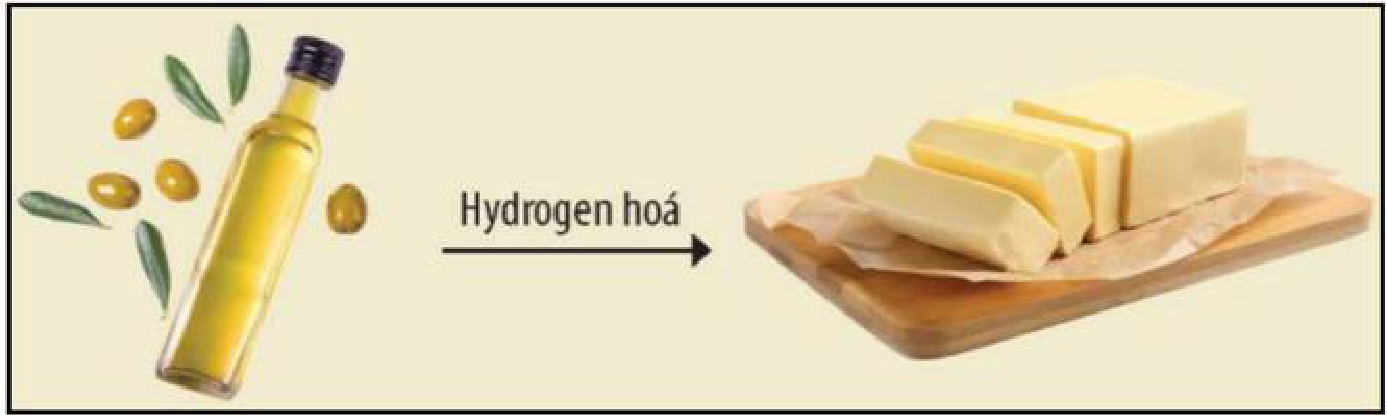
\includegraphics[width=9.5cm]{images_crop_de03/cau1_hydrogen_hoa_dau_an.png}
\end{center}
\choiceTF[t]
{Trong công nghiệp, người ta sử dụng phản ứng này để chuyển hóa chất béo lỏng thành chất béo rắn và ngược lại.}
{1 mol triolein (chất béo dạng lỏng) phản ứng tối đa với 3 mol $\ce{H2}$ (Ni, $t^\circ$) tạo thành tristearin (chất béo dạng rắn).}
{Do chứa các liên kết đôi ($\ce{C=C}$) trong phân tử, nên chất béo không no bị oxi hóa chậm bởi oxygen trong không khí tạo ra các chất có mùi khó chịu, làm cho dầu mỡ bị ôi.}
{Số nguyên tử carbon ở chất béo lỏng và rắn khác nhau.}
\loigiai{}
\end{ex}

\begin{ex}
Aspirin được sử dụng làm thuốc giảm đau, hạ sốt. Sau khi uống, aspirin bị thuỷ phân trong cơ thể tạo thành salicylic acid. Salicylic acid ức chế quá trình sinh tổng hợp prostaglandin (chất gây đau, sốt và viêm khi nồng độ trong máu cao hơn mức bình thường).
\begin{center}
	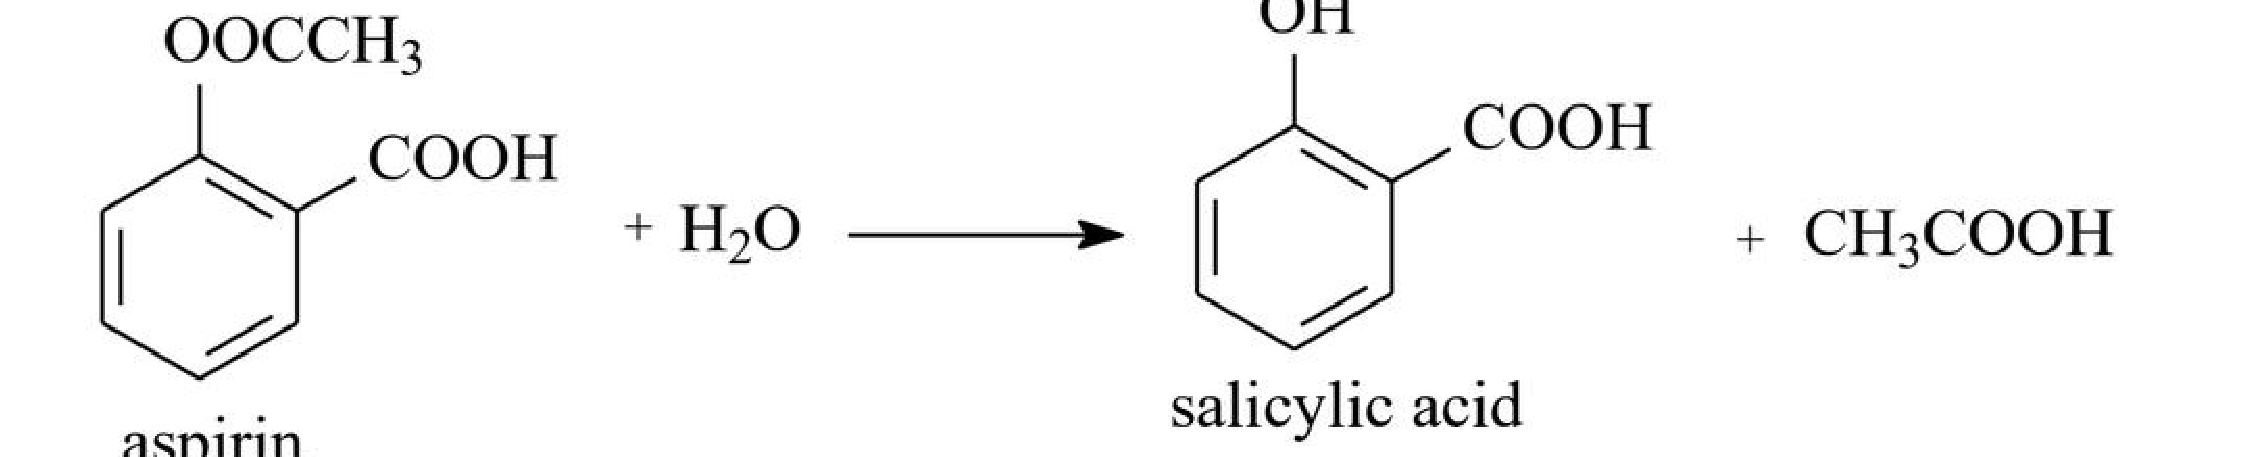
\includegraphics[width=11cm]{images_crop_de03/cau2_thuy_phan_aspirin.png}
\end{center}
\choiceTF[t]
{Aspirin có công thức phân tử $\ce{C9H8O4}$.}
{Salicylic acid có công thức phân tử $\ce{C7H6O3}$.}
{Aspirin có độ bất bão hòa $k = 5$.}
{Salicylic acid là hợp chất hữu cơ đa chức.}
\loigiai{}
\end{ex}

\begin{ex}
(SBT - CTST). Cho các chất sau:
\begin{center}
	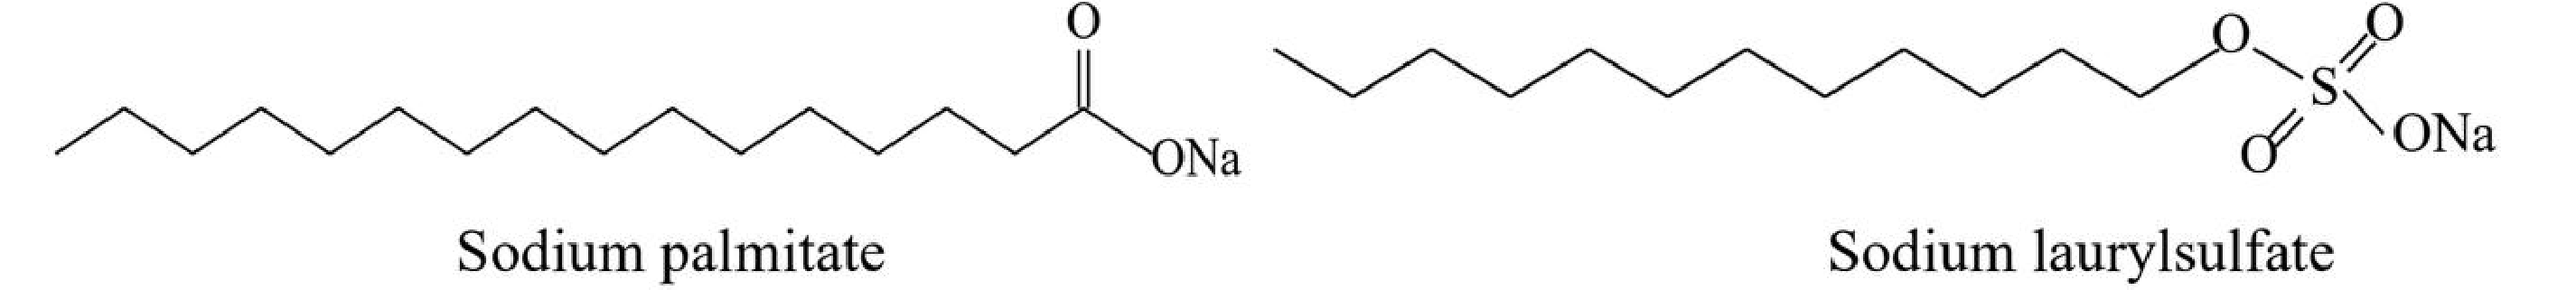
\includegraphics[width=12cm]{images_crop_de03/cau3_sodium_palmitate_laurylsulfate.png}
\end{center}
Xét tính đúng/sai của các phát biểu sau:
\choiceTF[t]
{Sodium palmitate và sodium laurylsulfate đều là thành phần chính của xà phòng.}
{Sodium palmitate và sodium laurylsulfate đều có tính năng giặt rửa.}
{Sodium palmitate và sodium laurylsulfate đều tạo muối khó tan trong nước cứng.}
{Sodium palmitate và sodium laurylsulfate đều có đầu ưa nước gắn với đuôi kị nước.}
\loigiai{}
\end{ex}

\begin{ex}
Các chất béo có thể là chất lỏng hoặc rắn, có trong một số loại động thực vật.
\choiceTF[t]
{Tripalmitin là một loại chất béo không no có trong mỡ động vật và dầu cọ có công thức phân tử là $\ce{C51H98O6}$.}
{Tristearin thu được từ mỡ động vật là một sản phẩm phụ của chế biến thịt bò có công thức phân tử là $\ce{C57H110O6}$.}
{Triolein chiếm 4-30\% trong dầu oliu là chất béo không no ở trạng thái lỏng có công thức là $\ce{C57H104O6}$.}
{Glyceryl trilinoleate hay trilinolein là chất béo no ở trạng thái rắn có công thức phân tử là $\ce{C57H98O6}$.}
\loigiai{}
\end{ex}

\vspace{0.3cm}
\noindent
\textbf{PHẦN III (1,5 điểm -- 6 câu): Câu trắc nghiệm yêu cầu trả lời ngắn.}\\
\textit{Thí sinh trả lời từ câu 1 đến câu 6. Mỗi câu hỏi thí sinh điền câu trả lời ngắn gọn theo yêu cầu.}

\setcounter{ex}{0}

\begin{ex}
(SBT - CTST). Có bao nhiêu ester của methyl alcohol có công thức phân tử là $\ce{C5H10O2}$?
\loigiai{}
\end{ex}

\begin{ex}
(SBT - CTST). Có bao nhiêu triglyceride mà khi xà phòng hoá hoàn toàn thu được glycerol cùng hỗn hợp chỉ gồm muối của palmitic acid và stearic acid?
\loigiai{}
\end{ex}

\begin{ex}
(SBT - KNTT). Xà phòng hoá hoàn toàn $4{,}4\text{ g}$ ethyl acetate bằng dung dịch $\ce{NaOH}$ dư, thu được bao nhiêu gam muối sodium acetate?
\loigiai{}
\end{ex}

\begin{ex}
(SBT - KNTT). Thực hiện phản ứng xà phòng hoá $100\text{ kg}$ chất béo chứa 80\% tristearin, còn lại là các tạp chất không phản ứng, thu được bao nhiêu kilogam sodium stearate? (Biết hiệu suất phản ứng xà phòng hoá là 90\%.) \textit{(Làm tròn kết quả đến hàng phần mười)}.
\loigiai{}
\end{ex}

\begin{ex}
Một loại chất béo có chứa 70\% triolein về khối lượng. Xà phòng hóa hoàn toàn $24\text{ kg}$ chất béo này trong dung dịch $\ce{NaOH}$, đun nóng thu được $x$ bánh xà phòng. Biết rằng trong mỗi bánh xà phòng có chứa $60\text{ gam}$ sodium oleate. Giá trị của $x$ là (lấy phần nguyên). Biết hiệu suất phản ứng đạt 90\%.
\loigiai{}
\end{ex}

\begin{ex}
Một loại chất béo có chứa 80\% tristearin về khối lượng. Để sản xuất 10 triệu chai nước rửa tay (có chứa chất dưỡng ẩm glycerol) cần dùng tối thiểu $x\text{ tấn}$ loại chất béo trên cho phản ứng với dung dịch $\ce{NaOH}$, đun nóng. Biết rằng trong mỗi chai nước rửa tay có chứa $6\text{ gam}$ glycerol. Giá trị của $x$ là \textit{(làm tròn kết quả đến hàng phần mười)}. Biết hiệu suất phản ứng đạt 75\%.
\loigiai{}
\end{ex}


\begin{center}
	\textbf{---------- HẾT ----------}
\end{center}

\end{document}
